% generated by Plantuml 1.2022.7       
\definecolor{plantucolor0000}{RGB}{241,241,241}
\definecolor{plantucolor0001}{RGB}{24,24,24}
\definecolor{plantucolor0002}{RGB}{169,220,223}
\definecolor{plantucolor0003}{RGB}{0,0,0}
\definecolor{plantucolor0004}{RGB}{132,190,132}
\definecolor{plantucolor0005}{RGB}{3,128,72}
\definecolor{plantucolor0006}{RGB}{255,255,68}
\definecolor{plantucolor0007}{RGB}{179,141,34}
\definecolor{plantucolor0008}{RGB}{173,209,178}
\definecolor{plantucolor0009}{RGB}{200,41,48}
\definecolor{plantucolor0010}{RGB}{242,77,92}
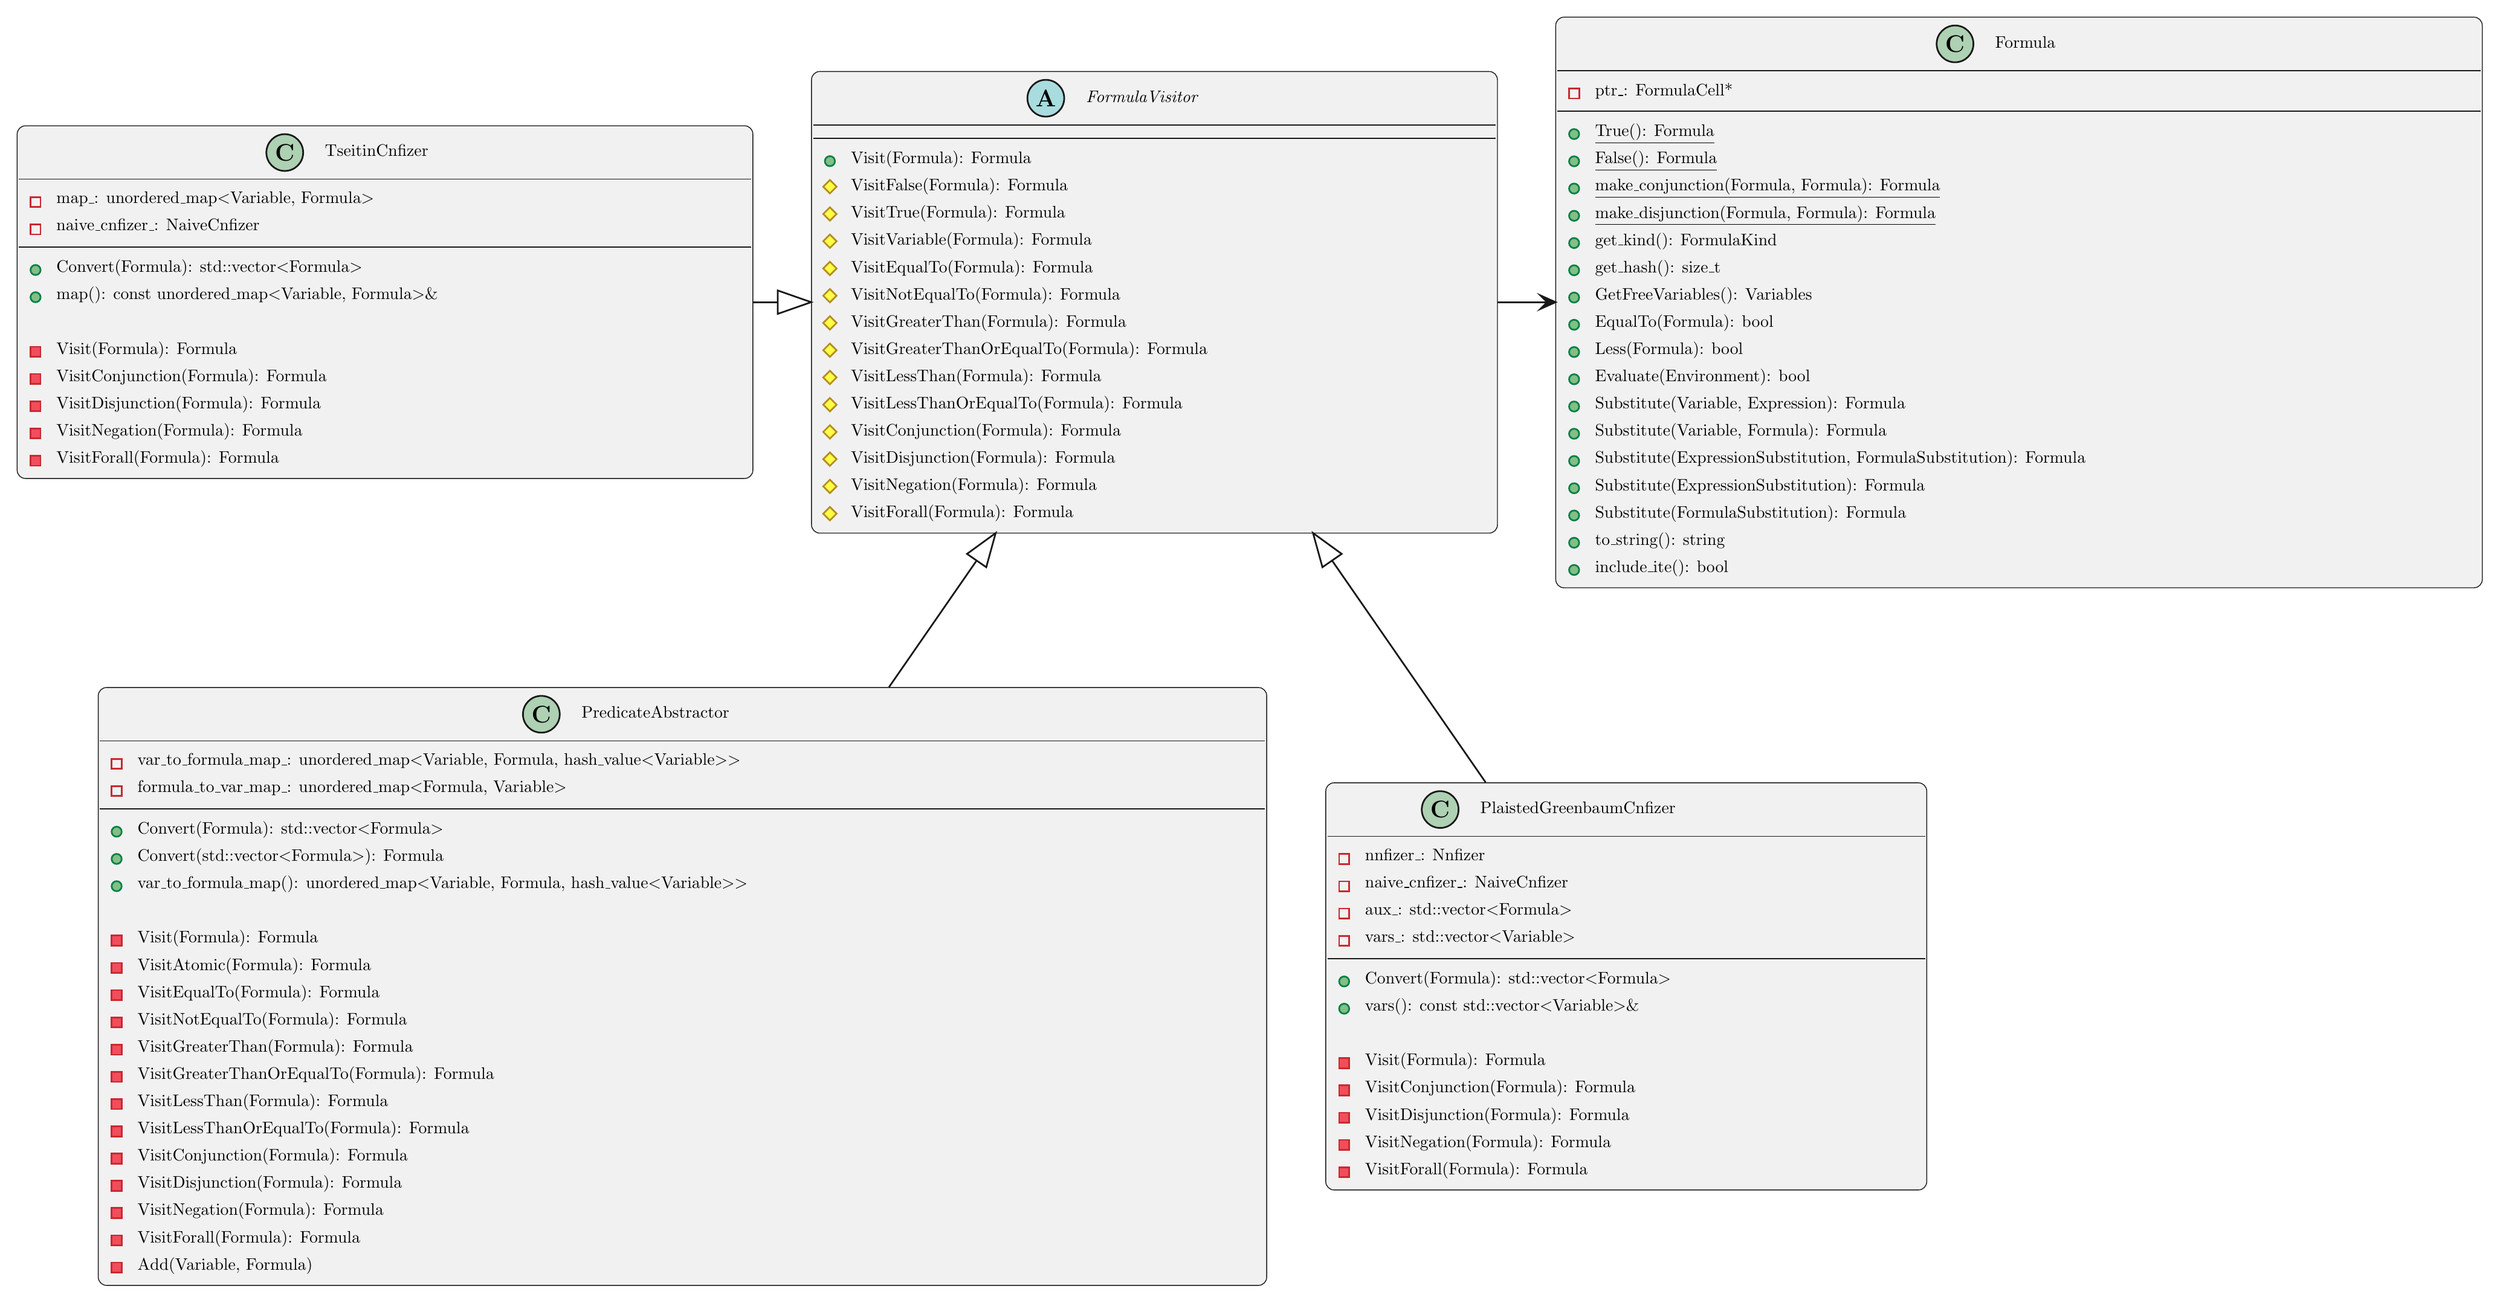
\begin{tikzpicture}[yscale=-1
,pstyle0/.style={color=plantucolor0001,fill=plantucolor0000,line width=0.5pt}
,pstyle2/.style={color=plantucolor0001,line width=0.5pt}
,pstyle3/.style={color=plantucolor0005,fill=plantucolor0004,line width=1.0pt}
,pstyle4/.style={color=plantucolor0007,fill=plantucolor0006,line width=1.0pt}
,pstyle5/.style={color=plantucolor0001,fill=plantucolor0008,line width=1.0pt}
,pstyle6/.style={color=plantucolor0009,line width=1.0pt}
,pstyle7/.style={color=plantucolor0009,fill=plantucolor0010,line width=1.0pt}
,pstyle8/.style={color=plantucolor0001,line width=1.0pt}
]
\draw[pstyle0] (482pt,44.5pt) arc (180:270:5pt) -- (487pt,39.5pt) -- (887.1524pt,39.5pt) arc (270:360:5pt) -- (892.1524pt,44.5pt) -- (892.1524pt,310.6563pt) arc (0:90:5pt) -- (887.1524pt,315.6563pt) -- (487pt,315.6563pt) arc (90:180:5pt) -- (482pt,310.6563pt) -- cycle;
\draw[color=plantucolor0001,fill=plantucolor0002,line width=1.0pt] (622.0929pt,55.5pt) ellipse (11pt and 11pt);
\node at (622.0929pt,55.5pt)[]{\textbf{\Large A}};
\node at (642.5929pt,47.3516pt)[below right,color=black]{\textit{FormulaVisitor}};
\draw[pstyle2] (483pt,71.5pt) -- (891.1524pt,71.5pt);
\draw[pstyle2] (483pt,79.5pt) -- (891.1524pt,79.5pt);
\draw[pstyle3] (493pt,93.1484pt) ellipse (3pt and 3pt);
\node at (502pt,83.5pt)[below right,color=black]{Visit(Formula): Formula};
\draw[pstyle4] (493pt,104.4453pt) -- (497pt,108.4453pt) -- (493pt,112.4453pt) -- (489pt,108.4453pt) -- cycle;
\node at (502pt,99.7969pt)[below right,color=black]{VisitFalse(Formula): Formula};
\draw[pstyle4] (493pt,120.7422pt) -- (497pt,124.7422pt) -- (493pt,128.7422pt) -- (489pt,124.7422pt) -- cycle;
\node at (502pt,116.0938pt)[below right,color=black]{VisitTrue(Formula): Formula};
\draw[pstyle4] (493pt,137.0391pt) -- (497pt,141.0391pt) -- (493pt,145.0391pt) -- (489pt,141.0391pt) -- cycle;
\node at (502pt,132.3906pt)[below right,color=black]{VisitVariable(Formula): Formula};
\draw[pstyle4] (493pt,153.3359pt) -- (497pt,157.3359pt) -- (493pt,161.3359pt) -- (489pt,157.3359pt) -- cycle;
\node at (502pt,148.6875pt)[below right,color=black]{VisitEqualTo(Formula): Formula};
\draw[pstyle4] (493pt,169.6328pt) -- (497pt,173.6328pt) -- (493pt,177.6328pt) -- (489pt,173.6328pt) -- cycle;
\node at (502pt,164.9844pt)[below right,color=black]{VisitNotEqualTo(Formula): Formula};
\draw[pstyle4] (493pt,185.9297pt) -- (497pt,189.9297pt) -- (493pt,193.9297pt) -- (489pt,189.9297pt) -- cycle;
\node at (502pt,181.2813pt)[below right,color=black]{VisitGreaterThan(Formula): Formula};
\draw[pstyle4] (493pt,202.2266pt) -- (497pt,206.2266pt) -- (493pt,210.2266pt) -- (489pt,206.2266pt) -- cycle;
\node at (502pt,197.5781pt)[below right,color=black]{VisitGreaterThanOrEqualTo(Formula): Formula};
\draw[pstyle4] (493pt,218.5234pt) -- (497pt,222.5234pt) -- (493pt,226.5234pt) -- (489pt,222.5234pt) -- cycle;
\node at (502pt,213.875pt)[below right,color=black]{VisitLessThan(Formula): Formula};
\draw[pstyle4] (493pt,234.8203pt) -- (497pt,238.8203pt) -- (493pt,242.8203pt) -- (489pt,238.8203pt) -- cycle;
\node at (502pt,230.1719pt)[below right,color=black]{VisitLessThanOrEqualTo(Formula): Formula};
\draw[pstyle4] (493pt,251.1172pt) -- (497pt,255.1172pt) -- (493pt,259.1172pt) -- (489pt,255.1172pt) -- cycle;
\node at (502pt,246.4688pt)[below right,color=black]{VisitConjunction(Formula): Formula};
\draw[pstyle4] (493pt,267.4141pt) -- (497pt,271.4141pt) -- (493pt,275.4141pt) -- (489pt,271.4141pt) -- cycle;
\node at (502pt,262.7656pt)[below right,color=black]{VisitDisjunction(Formula): Formula};
\draw[pstyle4] (493pt,283.7109pt) -- (497pt,287.7109pt) -- (493pt,291.7109pt) -- (489pt,287.7109pt) -- cycle;
\node at (502pt,279.0625pt)[below right,color=black]{VisitNegation(Formula): Formula};
\draw[pstyle4] (493pt,300.0078pt) -- (497pt,304.0078pt) -- (493pt,308.0078pt) -- (489pt,304.0078pt) -- cycle;
\node at (502pt,295.3594pt)[below right,color=black]{VisitForall(Formula): Formula};
\draw[pstyle0] (55.5pt,413pt) arc (180:270:5pt) -- (60.5pt,408pt) -- (749.1973pt,408pt) arc (270:360:5pt) -- (754.1973pt,413pt) -- (754.1973pt,760.6406pt) arc (0:90:5pt) -- (749.1973pt,765.6406pt) -- (60.5pt,765.6406pt) arc (90:180:5pt) -- (55.5pt,760.6406pt) -- cycle;
\draw[pstyle5] (320.4486pt,424pt) ellipse (11pt and 11pt);
\node at (320.4486pt,424pt)[]{\textbf{\Large C}};
\node at (340.9486pt,415.8516pt)[below right,color=black]{PredicateAbstractor};
\draw[pstyle2] (56.5pt,440pt) -- (753.1973pt,440pt);
\draw[pstyle6] (63.5pt,450.6484pt) rectangle (69.5pt,456.6484pt);
\node at (75.5pt,444pt)[below right,color=black]{var\_to\_formula\_map\_: unordered\_map\textless Variable, Formula, hash\_value\textless Variable\textgreater \textgreater };
\draw[pstyle6] (63.5pt,466.9453pt) rectangle (69.5pt,472.9453pt);
\node at (75.5pt,460.2969pt)[below right,color=black]{formula\_to\_var\_map\_: unordered\_map\textless Formula, Variable\textgreater };
\draw[pstyle2] (56.5pt,480.5938pt) -- (753.1973pt,480.5938pt);
\draw[pstyle3] (66.5pt,494.2422pt) ellipse (3pt and 3pt);
\node at (75.5pt,484.5938pt)[below right,color=black]{Convert(Formula): std::vector\textless Formula\textgreater };
\draw[pstyle3] (66.5pt,510.5391pt) ellipse (3pt and 3pt);
\node at (75.5pt,500.8906pt)[below right,color=black]{Convert(std::vector\textless Formula\textgreater ): Formula};
\draw[pstyle3] (66.5pt,526.8359pt) ellipse (3pt and 3pt);
\node at (75.5pt,517.1875pt)[below right,color=black]{var\_to\_formula\_map(): unordered\_map\textless Variable, Formula, hash\_value\textless Variable\textgreater \textgreater };
\node at (75.5pt,533.4844pt)[below right,color=black]{ };
\draw[pstyle7] (63.5pt,556.4297pt) rectangle (69.5pt,562.4297pt);
\node at (75.5pt,549.7813pt)[below right,color=black]{Visit(Formula): Formula};
\draw[pstyle7] (63.5pt,572.7266pt) rectangle (69.5pt,578.7266pt);
\node at (75.5pt,566.0781pt)[below right,color=black]{VisitAtomic(Formula): Formula};
\draw[pstyle7] (63.5pt,589.0234pt) rectangle (69.5pt,595.0234pt);
\node at (75.5pt,582.375pt)[below right,color=black]{VisitEqualTo(Formula): Formula};
\draw[pstyle7] (63.5pt,605.3203pt) rectangle (69.5pt,611.3203pt);
\node at (75.5pt,598.6719pt)[below right,color=black]{VisitNotEqualTo(Formula): Formula};
\draw[pstyle7] (63.5pt,621.6172pt) rectangle (69.5pt,627.6172pt);
\node at (75.5pt,614.9688pt)[below right,color=black]{VisitGreaterThan(Formula): Formula};
\draw[pstyle7] (63.5pt,637.9141pt) rectangle (69.5pt,643.9141pt);
\node at (75.5pt,631.2656pt)[below right,color=black]{VisitGreaterThanOrEqualTo(Formula): Formula};
\draw[pstyle7] (63.5pt,654.2109pt) rectangle (69.5pt,660.2109pt);
\node at (75.5pt,647.5625pt)[below right,color=black]{VisitLessThan(Formula): Formula};
\draw[pstyle7] (63.5pt,670.5078pt) rectangle (69.5pt,676.5078pt);
\node at (75.5pt,663.8594pt)[below right,color=black]{VisitLessThanOrEqualTo(Formula): Formula};
\draw[pstyle7] (63.5pt,686.8047pt) rectangle (69.5pt,692.8047pt);
\node at (75.5pt,680.1563pt)[below right,color=black]{VisitConjunction(Formula): Formula};
\draw[pstyle7] (63.5pt,703.1016pt) rectangle (69.5pt,709.1016pt);
\node at (75.5pt,696.4531pt)[below right,color=black]{VisitDisjunction(Formula): Formula};
\draw[pstyle7] (63.5pt,719.3984pt) rectangle (69.5pt,725.3984pt);
\node at (75.5pt,712.75pt)[below right,color=black]{VisitNegation(Formula): Formula};
\draw[pstyle7] (63.5pt,735.6953pt) rectangle (69.5pt,741.6953pt);
\node at (75.5pt,729.0469pt)[below right,color=black]{VisitForall(Formula): Formula};
\draw[pstyle7] (63.5pt,751.9922pt) rectangle (69.5pt,757.9922pt);
\node at (75.5pt,745.3438pt)[below right,color=black]{Add(Variable, Formula)};
\draw[pstyle0] (7pt,77pt) arc (180:270:5pt) -- (12pt,72pt) -- (441.9541pt,72pt) arc (270:360:5pt) -- (446.9541pt,77pt) -- (446.9541pt,277.9688pt) arc (0:90:5pt) -- (441.9541pt,282.9688pt) -- (12pt,282.9688pt) arc (90:180:5pt) -- (7pt,277.9688pt) -- cycle;
\draw[pstyle5] (167.0291pt,88pt) ellipse (11pt and 11pt);
\node at (167.0291pt,88pt)[]{\textbf{\Large C}};
\node at (187.5291pt,79.8516pt)[below right,color=black]{TseitinCnfizer};
\draw[pstyle2] (8pt,104pt) -- (445.9541pt,104pt);
\draw[pstyle6] (15pt,114.6484pt) rectangle (21pt,120.6484pt);
\node at (27pt,108pt)[below right,color=black]{map\_: unordered\_map\textless Variable, Formula\textgreater };
\draw[pstyle6] (15pt,130.9453pt) rectangle (21pt,136.9453pt);
\node at (27pt,124.2969pt)[below right,color=black]{naive\_cnfizer\_: NaiveCnfizer};
\draw[pstyle2] (8pt,144.5938pt) -- (445.9541pt,144.5938pt);
\draw[pstyle3] (18pt,158.2422pt) ellipse (3pt and 3pt);
\node at (27pt,148.5938pt)[below right,color=black]{Convert(Formula): std::vector\textless Formula\textgreater };
\draw[pstyle3] (18pt,174.5391pt) ellipse (3pt and 3pt);
\node at (27pt,164.8906pt)[below right,color=black]{map(): const unordered\_map\textless Variable, Formula\textgreater \&};
\node at (27pt,181.1875pt)[below right,color=black]{ };
\draw[pstyle7] (15pt,204.1328pt) rectangle (21pt,210.1328pt);
\node at (27pt,197.4844pt)[below right,color=black]{Visit(Formula): Formula};
\draw[pstyle7] (15pt,220.4297pt) rectangle (21pt,226.4297pt);
\node at (27pt,213.7813pt)[below right,color=black]{VisitConjunction(Formula): Formula};
\draw[pstyle7] (15pt,236.7266pt) rectangle (21pt,242.7266pt);
\node at (27pt,230.0781pt)[below right,color=black]{VisitDisjunction(Formula): Formula};
\draw[pstyle7] (15pt,253.0234pt) rectangle (21pt,259.0234pt);
\node at (27pt,246.375pt)[below right,color=black]{VisitNegation(Formula): Formula};
\draw[pstyle7] (15pt,269.3203pt) rectangle (21pt,275.3203pt);
\node at (27pt,262.6719pt)[below right,color=black]{VisitForall(Formula): Formula};
\draw[pstyle0] (789.5pt,470pt) arc (180:270:5pt) -- (794.5pt,465pt) -- (1143.8562pt,465pt) arc (270:360:5pt) -- (1148.8562pt,470pt) -- (1148.8562pt,703.5625pt) arc (0:90:5pt) -- (1143.8562pt,708.5625pt) -- (794.5pt,708.5625pt) arc (90:180:5pt) -- (789.5pt,703.5625pt) -- cycle;
\draw[pstyle5] (857.9071pt,481pt) ellipse (11pt and 11pt);
\node at (857.9071pt,481pt)[]{\textbf{\Large C}};
\node at (878.4071pt,472.8516pt)[below right,color=black]{PlaistedGreenbaumCnfizer};
\draw[pstyle2] (790.5pt,497pt) -- (1147.8562pt,497pt);
\draw[pstyle6] (797.5pt,507.6484pt) rectangle (803.5pt,513.6484pt);
\node at (809.5pt,501pt)[below right,color=black]{nnfizer\_: Nnfizer};
\draw[pstyle6] (797.5pt,523.9453pt) rectangle (803.5pt,529.9453pt);
\node at (809.5pt,517.2969pt)[below right,color=black]{naive\_cnfizer\_: NaiveCnfizer};
\draw[pstyle6] (797.5pt,540.2422pt) rectangle (803.5pt,546.2422pt);
\node at (809.5pt,533.5938pt)[below right,color=black]{aux\_: std::vector\textless Formula\textgreater };
\draw[pstyle6] (797.5pt,556.5391pt) rectangle (803.5pt,562.5391pt);
\node at (809.5pt,549.8906pt)[below right,color=black]{vars\_: std::vector\textless Variable\textgreater };
\draw[pstyle2] (790.5pt,570.1875pt) -- (1147.8562pt,570.1875pt);
\draw[pstyle3] (800.5pt,583.8359pt) ellipse (3pt and 3pt);
\node at (809.5pt,574.1875pt)[below right,color=black]{Convert(Formula): std::vector\textless Formula\textgreater };
\draw[pstyle3] (800.5pt,600.1328pt) ellipse (3pt and 3pt);
\node at (809.5pt,590.4844pt)[below right,color=black]{vars(): const std::vector\textless Variable\textgreater \&};
\node at (809.5pt,606.7813pt)[below right,color=black]{ };
\draw[pstyle7] (797.5pt,629.7266pt) rectangle (803.5pt,635.7266pt);
\node at (809.5pt,623.0781pt)[below right,color=black]{Visit(Formula): Formula};
\draw[pstyle7] (797.5pt,646.0234pt) rectangle (803.5pt,652.0234pt);
\node at (809.5pt,639.375pt)[below right,color=black]{VisitConjunction(Formula): Formula};
\draw[pstyle7] (797.5pt,662.3203pt) rectangle (803.5pt,668.3203pt);
\node at (809.5pt,655.6719pt)[below right,color=black]{VisitDisjunction(Formula): Formula};
\draw[pstyle7] (797.5pt,678.6172pt) rectangle (803.5pt,684.6172pt);
\node at (809.5pt,671.9688pt)[below right,color=black]{VisitNegation(Formula): Formula};
\draw[pstyle7] (797.5pt,694.9141pt) rectangle (803.5pt,700.9141pt);
\node at (809.5pt,688.2656pt)[below right,color=black]{VisitForall(Formula): Formula};
\draw[pstyle0] (927pt,12pt) arc (180:270:5pt) -- (932pt,7pt) -- (1476.0537pt,7pt) arc (270:360:5pt) -- (1481.0537pt,12pt) -- (1481.0537pt,343.3438pt) arc (0:90:5pt) -- (1476.0537pt,348.3438pt) -- (932pt,348.3438pt) arc (90:180:5pt) -- (927pt,343.3438pt) -- cycle;
\draw[pstyle5] (1165.7769pt,23pt) ellipse (11pt and 11pt);
\node at (1165.7769pt,23pt)[]{\textbf{\Large C}};
\node at (1186.2769pt,14.8516pt)[below right,color=black]{Formula};
\draw[pstyle2] (928pt,39pt) -- (1480.0537pt,39pt);
\draw[pstyle6] (935pt,49.6484pt) rectangle (941pt,55.6484pt);
\node at (947pt,43pt)[below right,color=black]{ptr\_: FormulaCell*};
\draw[pstyle2] (928pt,63.2969pt) -- (1480.0537pt,63.2969pt);
\draw[pstyle3] (938pt,76.9453pt) ellipse (3pt and 3pt);
\node at (947pt,67.2969pt)[below right,color=black]{\underline{True(): Formula}};
\draw[pstyle3] (938pt,93.2422pt) ellipse (3pt and 3pt);
\node at (947pt,83.5938pt)[below right,color=black]{\underline{False(): Formula}};
\draw[pstyle3] (938pt,109.5391pt) ellipse (3pt and 3pt);
\node at (947pt,99.8906pt)[below right,color=black]{\underline{make\_conjunction(Formula, Formula): Formula}};
\draw[pstyle3] (938pt,125.8359pt) ellipse (3pt and 3pt);
\node at (947pt,116.1875pt)[below right,color=black]{\underline{make\_disjunction(Formula, Formula): Formula}};
\draw[pstyle3] (938pt,142.1328pt) ellipse (3pt and 3pt);
\node at (947pt,132.4844pt)[below right,color=black]{get\_kind(): FormulaKind};
\draw[pstyle3] (938pt,158.4297pt) ellipse (3pt and 3pt);
\node at (947pt,148.7813pt)[below right,color=black]{get\_hash(): size\_t};
\draw[pstyle3] (938pt,174.7266pt) ellipse (3pt and 3pt);
\node at (947pt,165.0781pt)[below right,color=black]{GetFreeVariables(): Variables};
\draw[pstyle3] (938pt,191.0234pt) ellipse (3pt and 3pt);
\node at (947pt,181.375pt)[below right,color=black]{EqualTo(Formula): bool};
\draw[pstyle3] (938pt,207.3203pt) ellipse (3pt and 3pt);
\node at (947pt,197.6719pt)[below right,color=black]{Less(Formula): bool};
\draw[pstyle3] (938pt,223.6172pt) ellipse (3pt and 3pt);
\node at (947pt,213.9688pt)[below right,color=black]{Evaluate(Environment): bool};
\draw[pstyle3] (938pt,239.9141pt) ellipse (3pt and 3pt);
\node at (947pt,230.2656pt)[below right,color=black]{Substitute(Variable, Expression): Formula};
\draw[pstyle3] (938pt,256.2109pt) ellipse (3pt and 3pt);
\node at (947pt,246.5625pt)[below right,color=black]{Substitute(Variable, Formula): Formula};
\draw[pstyle3] (938pt,272.5078pt) ellipse (3pt and 3pt);
\node at (947pt,262.8594pt)[below right,color=black]{Substitute(ExpressionSubstitution, FormulaSubstitution): Formula};
\draw[pstyle3] (938pt,288.8047pt) ellipse (3pt and 3pt);
\node at (947pt,279.1563pt)[below right,color=black]{Substitute(ExpressionSubstitution): Formula};
\draw[pstyle3] (938pt,305.1016pt) ellipse (3pt and 3pt);
\node at (947pt,295.4531pt)[below right,color=black]{Substitute(FormulaSubstitution): Formula};
\draw[pstyle3] (938pt,321.3984pt) ellipse (3pt and 3pt);
\node at (947pt,311.75pt)[below right,color=black]{to\_string(): string};
\draw[pstyle3] (938pt,337.6953pt) ellipse (3pt and 3pt);
\node at (947pt,328.0469pt)[below right,color=black]{include\_ite(): bool};
\draw[pstyle8] (447.12pt,177.5pt) ..controls (451.99pt,177.5pt) and (456.87pt,177.5pt) .. (461.74pt,177.5pt);
\draw[pstyle8] (461.79pt,170.5pt) -- (481.79pt,177.5pt) -- (461.79pt,184.5pt) -- (461.79pt,170.5pt) -- cycle;
\draw[pstyle8] (793.38pt,332.22pt) ..controls (823.71pt,376.04pt) and (856.31pt,423.15pt) .. (885.09pt,464.75pt);
\draw[pstyle8] (787.51pt,336.04pt) -- (781.88pt,315.61pt) -- (799.02pt,328.07pt) -- (787.51pt,336.04pt) -- cycle;
\draw[pstyle8] (580.71pt,332.1pt) ..controls (563.61pt,356.8pt) and (545.79pt,382.56pt) .. (528.33pt,407.78pt);
\draw[pstyle8] (574.98pt,328.07pt) -- (592.12pt,315.61pt) -- (586.49pt,336.04pt) -- (574.98pt,328.07pt) -- cycle;
\draw[pstyle8] (892.23pt,177.5pt) ..controls (902.09pt,177.5pt) and (911.94pt,177.5pt) .. (921.79pt,177.5pt);
\draw[color=plantucolor0001,fill=plantucolor0001,line width=1.0pt] (926.94pt,177.5pt) -- (917.94pt,173.5pt) -- (921.94pt,177.5pt) -- (917.94pt,181.5pt) -- (926.94pt,177.5pt) -- cycle;
\end{tikzpicture}
